
\chapter{Problems with an Incompressibility Constraint}\label{chap6}

\section{Introduction}\label{chap6:ssec6.1} We\pageoriginale recall
the variational formulation of the Stokes problem (see Chapter
\ref{chap2}). 

Find $u\varepsilon V$ such that 
$$
a(u, v)=L(v) \; \forall\;v\varepsilon V,
$$
where
\begin{align*}
a(u, v) &= \int\limits_\Omega\nabla u.\nabla v\; dx,\\
L(v) &= \int\limits_\Omega f.v\;dx,\;f\varepsilon\;(L^2(\Omega))^n,
\end{align*}
and 
$$
V=\{v\varepsilon(H_\circ^1(\Omega))^n:\Div v=0\}.
$$

It is difficult to construct internal approximations of $V$ because of
the constraint $\Div v=0$. In two dimensional problem we know that 

$v\varepsilon V\Leftrightarrow$ there exists $\psi\varepsilon
H_\circ^2(\Omega)$ such that 
$$
v=\rot \psi,
$$
where 
$$
\rot \psi =\left(\frac{\partial\psi}{\partial x_2},-
\frac{\partial\psi}{\partial x_1}\right)
$$

Therefore, it seems logical that the difficulties we encountered in
approximating $H^2(\Omega)$ in a conforming way are transferred to the
conforming approximation of $V$.

\section{Approximation Via Finite Elements of Degree 1}\label{chap6:ssec6.2} Let\pageoriginale $W_h=\{v_h\;\varepsilon\;(C^\circ
(\overline{\Omega}))^2 :v_h|_K\;\varepsilon(\mathbb{P}_1(K))^2$, for
$K\varepsilon T_h, v_h=0$ on $\partial\Omega\}$ It is natural to try
for $V_h$ the space 
$$
\{v_h\;\varepsilon \;W_h: \Div\;v_h=0\}.
$$
But for most triangulations, $V_h=\{0\}$. This is due to the fact that
the number of equations due to the constraint $\Div v_h=0$ is greater
than the number of degrees of freedom of $W_h$. In fact,
$$
\text{Dimension of}\quad W_h=2\quad\text{($\#$ internal vertices)}.
$$
Number of equations due to the constraint $\Div v_h=0$ is equal to
number of triangles.

\noindent Hence $V_h$ cannot be a good approximation to $V$. However,
if the triangulation $T_h$ is obtained by first taking quadrilaterals
and then dividing each quadrilateral into four triangles by joining
the diagonals (see figure 6.1), we obtain a `good space' $V_h$. In
this case only 3 of the four equations $\Div v_h=0$ are independent. 
\begin{figure}[H]
\centering
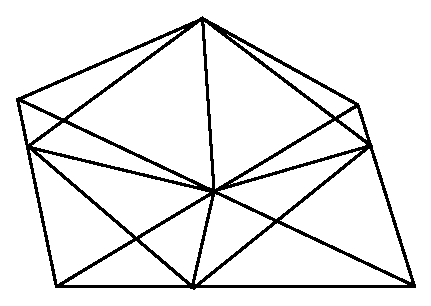
\includegraphics{figure/fig6.1.eps}
\caption{}\label{fig6.1}
\end{figure}

\setcounter{exercise}{0}
\begin{exercise}\label{chap6:exr1}
Let\pageoriginale $K$ be a quadrilateral. Let it be divided into four
triangles $T_i, 1\leq i\leq 4$, by 
\begin{figure}[H]
\centering
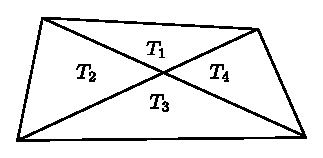
\includegraphics{figure/fig6.2.eps}
\caption{}\label{fig6.2}
\end{figure}
\noindent
joining the diagonals of $K$. Let $v\varepsilon C^\circ(\overline{K})$
such that 
$$
v|_{T_i}\;\varepsilon\mathbb{P}_1(T_i), 1\leq i\leq
4.\quad\text{Let}\quad d_i=\Div v|_{T_i}\;1\leq i\leq 4.
$$
Then show that $d_1+d_3=d_2+d_4$.

When the mesh is \emph{uniform}, it is possible to prove convergence
and to construct an interpolation operator,
$$
\pi_h:V\to V_h
$$
such that 
$$
\parallel v-\pi_h\;v\parallel_{1,\Omega}\leq \ch\parallel
v\parallel_{2,\Omega}.
$$
Therefore the solution $v_h$ of the approximate problem 
$$
a(u_h, v_h)=L(v_h)\;\; \forall\;v_h\;\varepsilon\;V_h,
$$
satisfies
$$
\parallel u-u_h\parallel_{1,\Omega}\leq\ch;\parallel
u-u_h\parallel_{0,\Omega}\leq \ch^2.
$$

When the domain is a square and the mesh is uniform we define $\pi_h$
as follows.

We choose for simplicity the diagonals of the square to be the
coordinate axes.
\begin{figure}[H]
\centering
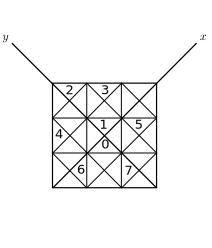
\includegraphics{figure/fig6.3.eps}
\caption{}\label{fig6.3}
\end{figure}\pageoriginale
\noindent
$\pi_hu$ at each of the main nodes (like 1, 5, 6, 7) is chosen as an
average of $u$. For example, at the node 1 the two components of
$\pi_hu$ are given by 
\begin{align*}
(\pi_hu)_1 &= \text{average of } u_1\text{ on } 02,\\
(\pi_hu)_2 &= \text{average of } u_2\text{ on } 34.
\end{align*}

At each of the secondary nodes (like 0, 2, 3, 4) $\pi_hu$ is chosen as
an average of the values of $\pi_hu$ at the main nodes. For example,
at the node $0$
\begin{align*}
(\pi_hu)_1\;(0) &= \frac{(\pi_hu)_1\;(1)+(\pi_hu)_1\;(7)}{2},\\
(\pi_hu)_2\;(0) &= \frac{(\pi_hu)_2\;(5)+(\pi_hu)_2\;(6)}{2},
\end{align*}

Numerically the method works even for irregular, not too distorted, meshes.
\end{exercise}

\section{The Fraeijs De Veubeke - Sander Element} \label{chap6:ssec6.3}
 We shall first describe a $C^1$ element of a non standard type: the Fraeijs de  Veubeke - Sander element.

Let\pageoriginale $K$ be a quadrilateral. We divide $K$ into four
triangles $T_i, 1\leq i\leq 4$, by joining the diagonals of $K$.
\begin{figure}[H]
\centering
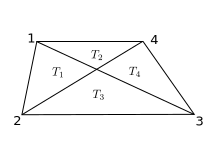
\includegraphics{figure/fig6.4.eps}
\caption{}\label{fig6.4}
\end{figure}

Let
$$
Q(K)=\{p\varepsilon C^1(K):p\varepsilon\mathbb{P}_3(T_i), 1\leq i\leq
4\}.
$$

We have 

\setcounter{lem}{0}
\begin{lem}\label{chap6:lem1}
$\dim Q(K)=16$.
\end{lem}
\begin{proof}
Indeed we choose $p=p_1$ on $T_1$ where
$p_1\varepsilon\mathbb{P}_3$. Then $p_1$ depends on 10 parameters. Let
$p_2 \varepsilon\mathbb{P}_3$ be such that $p_2$ and $\partial
p_2/\partial n$ vanish on the diagonal 13. Hence $p_2$ depends on
10-4-3=3 parameters. We choose $p=p_1+p_2$ on $T_2$ and it is easy to
see that $p$ is $C^1$ across 13.

In the same way we choose $p=p_1+p_3$ on $T_3$ with $p_3=\partial
p_3/\partial n=0$ on 24. $p_3$ depends again on 3 parameters and $p$
will be $C^1$ across 24.

Taking $p=p_1+p_2+p_3$ on $T_4$, it is easy to see that $p$ is $C^1$
across 13 and 24. Finally, $p$ depends on $10+3+3=16$
parameters. Hence the result.
\end{proof}

We\pageoriginale choose,
$$
\Sigma_K=\left\{\delta_i,\frac{\partial}{\partial x}\delta_i,
\frac{\partial}{\partial y}\delta_i, 1\leq i\leq 4;\frac{\partial}
{\partial n}\delta_{b_i},1\leq i\leq 4\right\}
$$
as the set of degrees of freedom. Here $b_i$ denotes the midpoint of a
side of the quadrilateral $K$.
\begin{figure}[H]
\centering
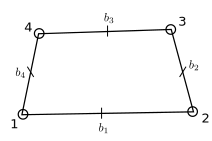
\includegraphics{figure/fig6.5.eps}
\caption{}\label{fig6.5}
\end{figure}

We refer the reader to CIAVALDINI-NEDELEC \cite{key11} to prove that this is
an admissible choice of degrees of freedom.

Let $Q_h$ denote a regular family of \emph{quadrangulations} of the
polygonal domain $\Omega$. Let 
$$
\chi_h=\{\phi_h\varepsilon C^1(\overline{\Omega}):\;\phi_h|_K\varepsilon
Q(K),\;\phi_h=\frac{\partial\phi_h}{\partial n}=0\quad\text{on}\quad
\partial\Omega\}.
$$
Then the following result has been proved by CIAVALDINI-NEDELEC \cite{key11}. 

\setcounter{THM}{1}
\begin{THM}\label{chap6:THM2}
The operator $\pi_h:H^3(\Omega)\to\chi_h$ defined by the above choice
of degrees of freedom satisfies
$$
\parallel\phi -\pi_h\phi\parallel_{2,\Omega}\leq\ch^s\parallel\phi
\parallel_{s+2,\Omega}, 
$$
where $s=1, 2$.
\end{THM}

As a consequence of this result the space $\chi_h$ can be
used\pageoriginale to approximate any variational problem on
$H_\circ^2(\Omega)$ and in particular the biharmonic problem
associated to the Stokes problem. However, as is the case with any
Hermite finite element, the programming of the Fde V-S element is
difficult and it is easier to use the corresponding element in the
velocity formulation, which is quadratic.

\section[Approximation of the Stokes Problem...]{Approximation of the
  Stokes Problem Via\hfil\break Quadratic 
  Elements}\label{chap6:ssec6.4}

Let $T_h$ be the triangulation associated to $Q_h$ by dividing each
quadrilateral of $Q_h$ into four triangles in the usual way. Let 
$$
W_h=\left\{v_h\;\varepsilon C^\circ(\overline{\Omega})^2:v_h|_T\;
\varepsilon(\mathbb{P}_2(T))^2,T\varepsilon T_h,v_h=0\quad\text{on}
\quad\partial\Omega\right\}  
$$
and 
$$
V_h=\{v_h\varepsilon W_h:\Div\; v_h=0\}.
$$

Obviously $v_h\varepsilon V_h$ implies that there exists $\psi_h
\varepsilon \chi_h$ such that $v_h=\rot\psi_h$. Therefore we can state

\begin{THM}\label{chap6:THM3}
There exists a constant $c$ such that, for $u\varepsilon V\cap
H^{s+1}(\Omega)$ ($s=1$ or $2$),
$$
\underset{v_h\varepsilon V_h}{\Inf}\parallel u-v_h\parallel_{1,\Omega}
\leq\ch^s\parallel u\parallel_{s+1,\Omega}.
$$
\end{THM}

\begin{proof}
As $u\varepsilon V$, there exists $\psi\varepsilon H^{s+2}(\Omega)\cap
H_\circ^2(\Omega)$ such that $u=\rot\psi$. Then choosing $v_h=\rot
\pi_h\psi$ we obtain the result. 
\end{proof}

Numerically,\pageoriginale one may solve the approximate problem:
\begin{equation*}
\begin{cases}
\text{find}\quad u_h\;\varepsilon V_h\quad\text{such that}\\
a(u_h, v_h)=L(v_h)\; \; \forall\;v_h\;\varepsilon V_h,
\end{cases}
\end{equation*}
via a penalty method.

Let $\varepsilon >0$ and
$$
a_\varepsilon\;(u, v)=a(u, v)+1/\varepsilon \int\limits_\Omega \Div\;
v \Div\; u\; dx.
$$
The penalised problem is:
\begin{equation*}
\begin{cases}
\text{Find}\quad u_h\;\varepsilon W_h\quad\text{such that}\\
a_\varepsilon(u_{\varepsilon h},v_h)=L(v_h)\; \; \forall \;v_h\;
\varepsilon W_h.
\end{cases}
\end{equation*}
This problem is much easier to solve. We shall see in Chapter
\ref{chap7} that the order of the error due to penalization is only 
$$
0(\varepsilon):\parallel u_{\varepsilon h}-u_h\parallel_1\leq
c.\varepsilon,
$$
where $c$ may depend on $h$.

\section{Penalty Methods.} \label{chap6:ssec6.5} We now come
back to the case of finite elements of degree 1 where the space $W_h$
is 
$$
W_h=\left\{v_h\;\varepsilon \;(C^\circ(\overline{\Omega}))^2:\;v_h|_K\;
\varepsilon \;(\mathbb{P}_1(K))^2, K\;\varepsilon \;T_h, v_h=0
\;\text{on}\; \partial \Omega\right\}.
$$
The approximate problem can be taken as 
\begin{equation*}
\begin{cases}
\text{Find}\quad u_{\varepsilon h}\;\varepsilon \;W_h\quad \text{such
that}\\
a_{\varepsilon}(u_{\varepsilon h}, v_h)=L(v_h)\quad\text{for all}\quad
v_h\;\varepsilon \;W_h.
\end{cases}
\end{equation*}
We have 

\begin{THM}\label{chap6:THM4}
Assume\pageoriginale that $u\varepsilon H^2(\Omega)$. Then there
exists a constant $c$ such that 
$$
\parallel u_{\varepsilon h}-u\parallel_1^2\leq c[h^2(1+1/\varepsilon)
+ h +\sqrt{\varepsilon}].
$$
Hence by choosing $\varepsilon =h^{4/3}$ we obtain
$$
\parallel u_{\varepsilon h}-u\parallel_1\leq\ch^{1/3}.
$$
\end{THM}

\begin{exercise}\label{chap6:exr2}
Prove the above theorem. 

Note that the above convergence rate is very poor, which is confirmed
by the poor numerical results obtained with this method.
\end{exercise}

\section{The Navier-Stokes Equations.} \label{chap6:ssec6.6}
The stationary flow of a viscous, Newtonian fluid subjected to gravity
loads in a bounded region $\Omega$ of $\mathbb{R}^3$ is governed by
the following dimensionless equations.
\begin{equation}\label{chap6:eq6.1}
\left.
\begin{aligned}
-\gamma\Delta u+\sum\limits_{i=1}^3u_i\frac{\partial u} {\partial x_i}
+\nabla p &= f\quad\text{in}\quad\Omega,\\
\Div u &= 0\quad\text{in}\quad\Omega,\\
u &= 0\quad\text{in}\quad\partial\Omega,
\end{aligned}
\right\}
\end{equation}
where $u$ represents the velocity, $p$ the pressure and $f$ is the
body force. All these quantities are in dimensionless form and $\gamma
=\frac{\mu}{DV_\rho}=\frac{1}{Re}$ where $Re$ is called the Reynolds
number. Here is the viscosity of the fluid $D$ a length characterizing
the domain\pageoriginale $\Omega,V$ a characteristic velocity of the
flow and $\rho$ the density of the fluid (For more details the reader
is referred to BIRD-STEWART-LIGHTFOOR `Transport Phenomena, Wiley
Ed. p. 108).

The Reynolds number is the only parameter in the equation and it
measures how far the Navier-Stokes model is from the Stokes model. The
limiting case $\gamma =0$ corresponds to Euler's equations for
inviscid fluids. However, at high Reynolds number, the flow develops a
boundary layer near the boundary. Moreover, instability and
bifurcation phenomena can be observed which correspond physically to
turbulence. We are going to study only the flows at \emph{low}
Reynolds number.

\section[Existence and Uniqueness of Solutions of...]{Existence and
  Uniqueness of Solutions of\hfil\break 
  Navier-Stokes}\label{chap6:ssec6.7}  

EQUATIONS AT LOW REYNOLDS NUMBERS. The variational formulation of
Navier-Stokes equations is:
\begin{equation}\label{chap6:eq6.2}
\begin{cases}
\text{Find}\quad u\varepsilon V\quad\text{such that}\\
a(u, v)+b(u, u, v)=(f, v)\; \; \forall v\varepsilon V,
\end{cases}
\end{equation}
where
\begin{equation*}
\begin{split}
a(u, v)=\gamma\int\limits_\Omega\nabla u.\nabla v\; dx,\\
b(u, v, w)=\int\limits_\Omega\sum\limits_{i,j=1}^3 u_i \frac{\partial
v_j}{\partial x_i}w_j\; dx
\end{split}
\end{equation*}
and
$$
V=\{v\varepsilon \;(H_\circ^1(\Omega))^3:\Div v=0\}.
$$

\begin{exercise}\label{chap6:exr3}
Show\pageoriginale that if $u$ is a solution of \eqref{chap6:eq6.2},
then there exists a $p\varepsilon L^2(\Omega)$ such that $\{u,p\}$ is
a solution of \eqref{chap6:eq6.1} in the sense of distributions. 
\end{exercise}

\begin{exercise}\label{chap6:exr4}
Show that for all $u, v, w \varepsilon V$ one has 
\begin{align*}
b(u, v, w) &= -b(u, w, v),\\
b(u, v, v) &= 0.
\end{align*}
\end{exercise}

As $H^1(\Omega)\hookrightarrow L^4(\Omega)$ (see LADYZHENSKAYA \cite{key27}
for a proof of this), using Schwarz inequality twice we obtain
$$
b(u,v,w)\leq\parallel u\parallel_{0,4}\parallel v\parallel_1\parallel
w\parallel_{0,4}\leq c\parallel u\parallel_1\parallel v\parallel_1
\parallel w\parallel_1.
$$
Hence
$$
\beta =\underset{u,v,w\varepsilon V}{\Sup} \frac{b(u,v,w)} {\parallel
u\parallel \parallel v\parallel \parallel w\parallel}<\infty.
$$
where $\parallel u\parallel =|u|_1$. We have 

\begin{THM}\label{chap6:THM5}
Assume that $\beta/\gamma^2\parallel f\parallel_* <1$. Then the
problem \eqref{chap6:eq6.2} has a unique solution.
\end{THM}

\begin{proof}
Let $u^i\varepsilon V, i=1,2$. Let $v^i, i=1,2$ be the solution
\begin{equation}\label{chap6:eq6.3}
a(v^i,w)+b(u^i,v^i,w)=(f,w)\; \; \forall w\varepsilon \;V\;i=1,2
\end{equation}
Note that \eqref{chap6:eq6.3} is a linear problem and has a unique
solution by virtue of the Lax-Milgram Lemma. 

Choosing\pageoriginale $w=v^i$ in \eqref{chap6:eq6.3} it is easy to
see that 
$$
\gamma\parallel v^i\parallel^2\leq(f,v^i)\leq\parallel
f\parallel_*\parallel v^i\parallel.,
$$
Thus 
$$
\parallel v^i\parallel \leq\frac{\parallel f\parallel_*}{\gamma}
$$
Taking $w=v^2-v^1$, we obtain
\begin{equation*}
\begin{split}
\gamma\parallel w\parallel^2\leq a(v^2-v^1,w)=b(u^1,v^1,w)-b(u^2,v^2,
w)=b(u^1,-w,w)+\\
+b(u^1-u^2,v^2,w)\leq 0+\beta\parallel v^2\parallel\centerdot\parallel
w\parallel \parallel u^1-u^2\parallel.
\end{split}
\end{equation*}
Hence we obtain
$$
\parallel v^1-v^2\parallel\leq\frac{\beta}{\gamma^2}\parallel
f\parallel_*\parallel u^1-u^2\parallel.
$$

Since $\frac{\beta}{\gamma^2}\parallel f\parallel_* <1$, the mapping
$T:u^i\to v^i$ is a strict contraction and has a fixed point which
obviously is the unique solution of \eqref{chap6:eq6.2}
\end{proof}

\setcounter{REM}{0}
\begin{REM}\label{chap6:rem1}
The proof is constructive in the sense that the algorithm
$u^{n+1}=Tu^n$ gives a sequence which converges to the solution. At
each step of this algorithm one has to solve the linearised problem
\eqref{chap6:eq6.3}. 
\end{REM}

\begin{REM}\label{chap6:rem2}
If $\gamma^2\geq\beta\parallel f\parallel_*$ then there exists atleast
one solution to \eqref{chap6:eq6.2}. The solution of
\eqref{chap6:eq6.2} in this case may not be unique (see LIONS
\cite{key28}). Note that problem \eqref{chap6:eq6.2} is equivalent
to\pageoriginale solving a non-linear equation $F(u)=0$ where $F:V\to
V'$ is given by
$$
F(u)(v)=a(u,v)+b(u,u,v)-(f,v).
$$
Let $G_u$ be the linear operator which is tangent to $F$, \ie 
$$
(G_u w,v)=\lim\limits_{\theta\to 0}\frac{1}{\theta}(F(u+\theta
w)-F(u),v)=a(w,v)+b(u,w,v)+b(w,u,v).
$$
If $G_u$ is not singular, then $u$ is an isolated solution, otherwise
there may be a bifurcation. The eigenvalue problem associated to the
linearised problem is: 
\begin{equation*}
\begin{cases}
\text{Find}\quad w\varepsilon V,\lambda\;\varepsilon \not\kern -3pt C
\quad\text{such that}\\
a(w,v)+b(u,w,v)+b(w,u,v)=\lambda(w,v)\; \; v\;\varepsilon V
\end{cases}
\end{equation*}
and a study of this problem is of fundamental interest.

We refer the reader to BREZZI-RAPPAZ-RAVIART \cite{key6} for a study of the
convergence in the case where $u$ is an isolated solution. In the next
section we restrict ourselves to the case where $u$ is unique.
\end{REM}

\section{Error Estimates for Conforming  Method} \label{chap6:ssec6.8} 
Let $V_h\subset V$. We consider the approximate problem:
\begin{equation}\label{chap6:eq6.4}
\begin{cases}
\text{Find}\quad u_h\;\varepsilon V_h\quad\text{such that}\\
a(u_h,v_h)+b(u_h,u_h,v_h)=(f,v_h) \; \forall\;v_h\;\varepsilon\;V_h
\end{cases}
\end{equation}

Let
$$
\beta_h=\underset{u,v,w\varepsilon V_h}{\Sup}\frac{b(u,v,w)}
{\parallel u\parallel \parallel v\parallel \parallel w\parallel} 
$$
and\pageoriginale 
$$
\parallel f\parallel_{h*}=\underset{u\varepsilon V_h}{\Sup}
\frac{(f,v)}{\parallel v\parallel}.
$$
Then it is easy to see that \eqref{chap6:eq6.4} has a unique solution
when 
$$
\frac{\beta_h}{\gamma^2}\parallel f\parallel_{h*} <1.
$$
The iterative method mentioned in Remark \ref{chap6:rem1} converges
for all $\gamma$ satisfying $\gamma^2 >\beta_h\parallel
f\parallel_{h*}$ Note that $\beta_h\leq\beta$ and $\parallel
f\parallel_{h*}\leq\parallel f\parallel_*$; however, JAMET-RAVIART
\cite{key23} proved that $\beta_h\to\beta$ and $\parallel
f\parallel_{h*}\to\parallel f\parallel_*$ as $h\to 0$. 

\begin{THM}\label{chap6:THM6}
Assume that 
$$
\frac{\beta}{\gamma^2}\parallel f\parallel_* < 1-\delta
$$
with $0<\delta < 1$; then one has 
$$ 
\parallel u-u_h\parallel \leq 3/\delta\parallel u-v_h\parallel
\; \; \forall \; v_h\;\varepsilon V_h.
$$
\end{THM}

\begin{proof}
Let $w_h=v_h-u_h$. Then 
\begin{gather*}
\gamma\parallel w_h\parallel^2\leq a(v_h-u,w_h)+a(u-u_h,w_h),\\
a(u,w_h)=(f,w_h)-b(u,u,w_h),\\
a(u_h,w_h)=(f,w_h)-b(u_h,u_h,w_h),\\
a(u-u_h,w_h)=b(u_h,u_h-u,w_h)\\
+b(u_h-u,u,w_h)\leq\beta\parallel
u_h\parallel \parallel v_h-u\parallel \parallel w_h\parallel +
\beta\parallel u_h-u\parallel \centerdot \parallel u\parallel\\
\parallel
 w_h\parallel\quad\text{since}\quad b(u_h,u_h-v_h,w_h)=0.
\end{gather*}
But we know that 
$$
\parallel u\parallel\leq 1/\gamma\parallel f\parallel_*,\parallel
u_h\parallel \leq 1/\gamma\parallel f\parallel_*.
$$\pageoriginale
Therefore we obtain
$$
\parallel w_h\parallel^2 \leq\left(\parallel v_h-u\parallel
+(1-\delta)\parallel v_h-u\parallel +(1-\delta)\parallel
u_h-u\parallel\right).\parallel w_h\parallel.
$$
As 
$$
\parallel u-u_h\parallel\leq\parallel u-v_h\parallel +\parallel
w_h\parallel 
$$
we get
$$
\delta\parallel w_h\parallel^2\leq(3-2\delta)\parallel v_h-u\parallel
\parallel w_h\parallel.
$$
Hence
$$
\parallel u-u_h\parallel\leq\parallel v_h-u\parallel +\frac{3-2\delta}
{\delta}\parallel u-v_h\parallel.
$$
This gives the desired result.
\end{proof}

An immediate consequence of Theorem \ref{chap6:THM6} is that, when the
solution $u$ of \eqref{chap6:ssec6.2} is sufficiently regular, we
obtain the same error estimate for Navier-Stokes equations at low
Reynolds number as for Stokes.

The method described in Section \ref{chap6:ssec6.4} is probably one of
the best methods for Navier-Stokes equations at low Reynolds number.

However, when the Reynolds number is large, a major disadvantage is
that the velocity field is required to be continuous (since our method
is conforming) and this is not good to take into account boundary
layer phenomena.

Indeed\pageoriginale the velocity profile near the boundary has the
behaviour as shown in figure.
\begin{figure}[H]
\centering
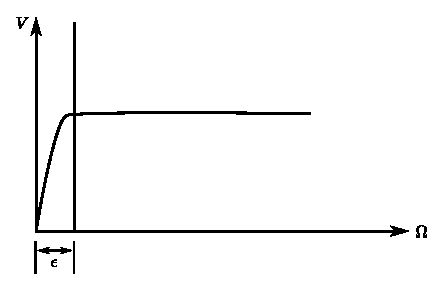
\includegraphics{figure/addfig6.6.eps}
\caption{}\label{fig6.6}
\end{figure}
\noindent
$\in$ is called the thickness of the boundary layer. In fact,
$\in =\gamma^{1/2}$, so that for high Reynolds number, this
requires a very high refinement of the mesh near the boundary and
therefore very expensive computer time. This can be partly avoided
with mixed finite element since we shall work with discontinuous
velocity fields.


